\chapter{Introduction}

\lettrine{U}{ntil} the early 2000s Unmanned Aerial Vehicles (UAVs) were limited to the defense and military industries, because of the high costs and the complexity of constructing these vehicles. Nevertheless, they have become cheaper and more available in several civil and academic applications over the past decades. They have not just become more common, but their capabilities have dramatically increased, therefore they are more popular and widely used in applications such as rescue operations~\cite{rescue-operations}, data collection, and geophysics exploration~\cite{data-collection}, inspections~\cite{inspection}, and agricultural purposes~\cite{agriculure}.

This expansion required not only technical developments but also advancement in traditional navigation methods, where the Global Positioning System (GPS) is combined with the Inertial Navigation System (INS), creating a GPS-INS system~\cite{gps-ins}. The small unmanned aircraft's future impact depends on how well they can navigate in GPS-denied environments such as narrow city corridors or circumstances with GPS disturbance or spoofing.  Inertial measurements by themselves can be used to estimate the position of the aircraft respected to a known initial position, but they will accumulate errors over time, especially with low-cost Inertial Measurement Unit (IMU) sensors. The phenomenon is usually called drift because estimated values drift away from the true values with time.

To give a better estimation of the position in most GPS-free applications exteroceptive sensors are used such as cameras, laser scanners, distance sensors, \etc{} The type of used sensor mostly depends on the kind of vehicle. For example only considering UAVs, a multirotor drone has completely different aircraft dynamics, mission profile, and sensing requirements compared to fixed-wing aircraft. Since fixed-wing aircraft usually fly at high altitudes above the environment with relatively high speeds, distance sensors are ineffective. In this case, the most common approach is using cameras for instance, both~\cite{gps-ins-cam} and~\cite{rel-nav} leverage visual information captured by cameras and integrate this data with measurements from an IMU to estimate the motion of the aircraft. 

\section{Possible sources of global information}

When an algorithm fails to close the navigation loop, particularly in the absence of external absolute positioning references, it results in the estimates drift, which emerges due to the algorithm's inability to establish consistent and accurate reference points or constraints, thereby leading to unbounded cumulative errors over time.

Of course, the most straightforward solution to this problem is to use the signals of Global Navigation Satellite Systems (GNSS) such as the US GPS, the Russian GLONASS (Global Navigation Satellite System), the European Galileo~\cite{GNSS}, or the Chinese BDS (BeiDou Navigation Satellite System)~\cite{BeiDou}. The problem with these systems they are not always available for example, in indoor environments, the GPS signal can be shadowed, and in outdoor environments, it can be jammed or spoofed. 

Another solution is to use a map of the environment, which is usually called Simultaneous Localization and Mapping (SLAM)~\cite{SLAM}. The main idea behind SLAM is to estimate the position of the vehicle and the map of the environment simultaneously. The map can be used as a reference to correct the drift errors. The map can be built up by using the measurements of the exteroceptive sensors, such as cameras, laser scanners, \etc{} The problem with this approach is that the map can be built up only in the explored area, therefore it is not a solution for the first flight of the aircraft. 

The last remedy can involve leveraging Signals of Opportunity (SOPs), which are signals not originally intended for navigation but can be used for this purpose. In~\cite{SOP}, they propose SOPs can be terrestrial (\eg{}, FM radio, cellular, digital television) or space-based (\eg{}, Low Earth Orbit (LEO) satellites). In navigation, SOPs leverage known synchronization sequences or beacons from the used sources. These signals enable cognitive navigation by providing measurements like Time-of-Arrival (TOA), indicating signal travel time; Direction-of-Arrival (DOA), specifying signal direction; and Frequency-of-Arrival (FOA), denoting signal frequency~\cite{SOP-terrestrial}. In the case of LEO satellites, their broadband communication signals can be used for navigation~\cite{SOP-LEO}. 

\section{Relative navigation}

The measurement fusion and sensor noise filtering can take place in an Extended Kalman Filter (EKF) framework because typically these are nonlinear systems. EKFs can be used on any kind of vehicle including robots~\cite{EKF-Robot}, Unmanned Aerial Systems (UAS)~\cite{EKF-UAS-1, EKF-UAS-2}, \etc{} They can account for both sensor errors and process uncertainty, but it is important to note that these methods only work well when errors remain small \eg{} when the availability of GPS measurements makes it possible to regularly remove drift errors. When GPS or any other global measurements are unavailable for a longer period, the global position and yaw angle of the aircraft are unobservable, which eventually leads to the divergence of estimates~\cite{unobservable-1, unobservable-2}. In addition, if an EKF receives a global measurement after significant drift errors have accumulated, nonlinearities can complicate the utilization of the measurement, and it could result in large jumps in the estimate, in some cases it can even lead to filter divergence. This is because the local linearization of the measurement equations around the drifted states is applied, which can present incorrect dynamics.

In recent years a new method was proposed called relative navigation~\cite{rel-nav-1, rel-nav-2}, which can handle these observability and consistency problems. With exteroceptive sensors, the navigation can be performed concerning the surroundings, hence this method can be divided into a relative front end and a global back end, the complete architecture is shown in Figure~\ref{fig:real-nav}. 

\begin{figure}[H]
    \centering
    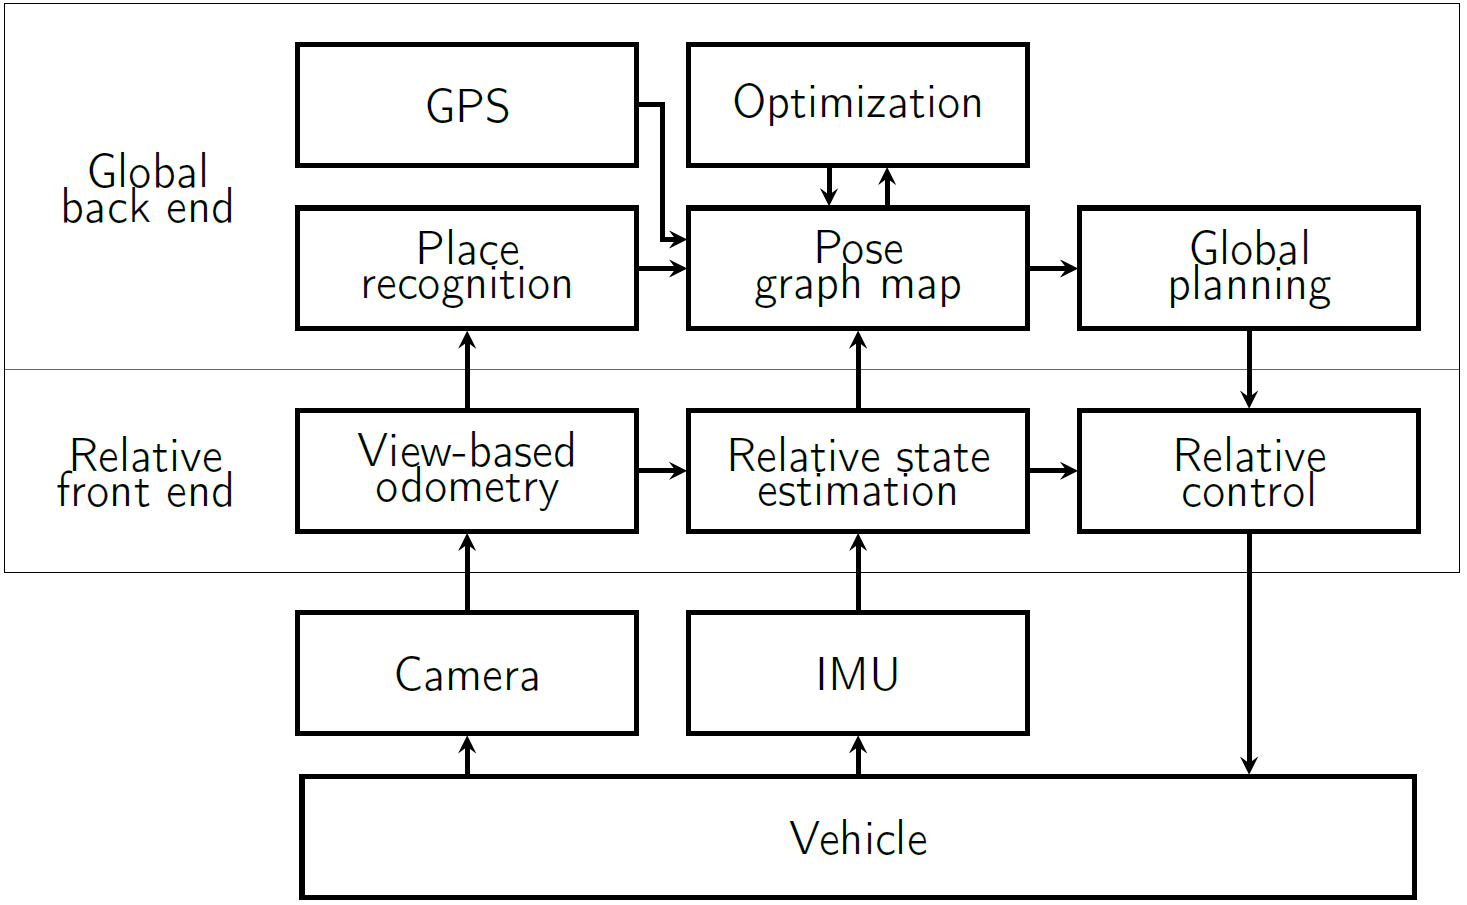
\includegraphics[width=0.7\textwidth]{figures/rel-nav}
    \caption{Block diagram of relative navigation (\cite{rel-nav}: page 2, Figure 2)}\label{fig:real-nav}
\end{figure}

The front end provides an estimation of the state relative to the local environment, while the back end is a mapping algorithm, which uses a pose graph based on the results of the front end to produce global estimates. Several important observability and computational benefits are obtained by dividing the architecture into a relative front end and a global back end:
\begin{itemize}
    \item 
    The front end calculates the estimate relative to a local frame, where the states can remain observable and the uncertainty can be accurately represented by a Gaussian distribution. This enables the utilization of the computational advantage of an Error-State Kalman Filter (ESKF), which is a better solution, than an ordinary EKF because it calculates the nominal (ideal) state according to the original non-linear dynamics and the linearization is performed on the so-called error state which is defined around the nominal state.
    
    \item 
     On the other hand, the back end uses a pose graph that can effectively represent nonlinearities in heading and can be robustly optimized with additional constraints, such as opportunistic global measurements or place recognition.
\end{itemize}

In this paper, a visual-inertial navigation algorithm will be presented. The target UAV is a fixed-wing aircraft called Sindy, shown in Figure~\ref{fig:sindy}.

\begin{figure}[!ht]
    \centering
    \includesvg[width=0.8\textwidth]{figures/Sindy}
    \caption{Realistic drawing of Sindy (\cite{sindy-manual}: title page)}\label{fig:sindy}
\end{figure}

\section{Structure of the paper}

To sum up the involved steps during the project, the primary objective was to integrate a visual-inertial ESKF into a simulation that was already available to me. The simulation contained a grid of feature points, and the goal was to use an ESKF-based algorithm to estimate the aircraft's state while flying along a predefined trajectory. I followed a gradual approach in the development process, starting with ideal conditions and incrementally introducing more realistic elements to the simulation. These included IMU- and measurement- noises, sensor biases, pixelization, and later the usage of real image processing algorithms. Firstly, I implemented the filter with known 3-D coordinates of the measured feature points, but later a triangulation method was implemented called Linear Optimal Sine Triangulation (LOST). The next step involved the integration of the two methods. 

The paper is structured as follows: Chapter~\ref{chap:math} provides an introduction to several fundamental mathematical concepts that are crucial for comprehending this approach. In Chapter~\ref{chap:eskf}, the mathematical foundations of the filter are explained, and the steps of the filter are detailed. Chapter~\ref{chap:LOST} focuses on the introduction of the applied triangulation method called LOST.\@ Chapter~\ref{chap:integration} is devoted to introducing the integration issues of ESKF and LOST.\@ Chapter~\ref{chap:dev} presents the results of the filter in the Matlab/Simulink simulation environment. Finally, Chapter~\ref{chap:conclusion} offers a summary of the work, and highlights certain future development steps.